% (c) 2020 Stefan Antonowicz
% Based off of tex found at https://github.com/ludus-leonis/nipajin
% This file is released under Creative Commons Attribution-NonCommercial-ShareAlike 4.0 International License.
% Please do not apply other licenses one-way.

\renewcommand{\yggAppendix}{%
  \mychapter{Appendices}{appendices}

    \begin{center}
    
\includegraphics[width=\linewidth,keepaspectratio=true]{appendices/ToyHeader2}
    \end{center}
    \newpage
  \newpage


}

\renewcommand{\yggAppendixText}{%

  \newpage
  \mysection{Appendix A: Goodies}{appendix-a}

\begin{multicols*}{2}

\mysubsection{Basic Treasure Table}{appendix-a-basic-treasure}

\mytable{l X}{
 \thead{d6} & \thead{}  \\
}{
 1 & Nothing \\
 2 & Mundane Treasure I \\
 3 & Mundane Treasure II \\
 4 & d6 coins \\
 5 & d6x10 coins \\
 6 & Roll on \mybold{Better Treasure Table}
}


\mysubsection{Better Treasure Table}{appendix-a-better-treasure}

\mytable{l X}{
 \thead{d6} & \thead{}  \\
}{
 1 & Roll on \mybold{Gems} \\
 2 & Roll on \mybold{Jewelry} \\
 3 & Choose or roll a random \mylink{Narcotic}{gear-narcotics} \\
 4 & Roll on \mybold{Chymistry} below \\
 5 & Roll on \mybold{Fetishes} below \\
 6 & Choose an appropriate \mylink{Marvel}{cunning-marvels}
}

\myimage{appendices/TreasureChest}


\cbreak

\mysubsection{Mundane Treasure I}{appendix-a-mundane-treasure-1}
\myital{Roll 2d6}


\mytable{l X} {
    \thead{} & \thead{} \\
}{
    11 & False Teeth \\
    12 & Obscure treasure map \\
    13 & Love Letter \\
    14 & Small silver knife \\
    15 & Set of rusty keys \\
    16 & Matches \\
    21 & Copper hand mirror \\
    22 & Spikes and a hammer \\
    23 & Syringe (empty) \\
    24 & Leather work gloves \\
    25 & Flask of oil \\
    26 & Flask of liquor \\
    31 & Chalk \\
    32 & 3 beans \\
    33 & Mousetrap \\
    34 & A few wooden puzzle pieces \\
    35 & A carved pipe \\
    36 & A rabbit's foot \\
    41 & A set of dice \\
    42 & Brass ring \\
    43 & 3 playing cards (Aces) \\
    44 & A children's toy top \\
    45 & Small bone statues \\
    46 & Blue quartz crystal \\
    51 & A pair of purple ladies gloves \\
    52 & A bag of teeth \\
    53 & A few bones \\
    54 & A comb \\
    55 & A handkerchief \\
    56 & Small petrified head \\
    61 & A few round stones \\
    62 & A wool cap \\
    63 & A pair of undarned socks \\
    64 & Small bottle of urine \\
    65 & A duck bill \\
    66 & A morbid shopping list (body parts) \\
}


\mysubsection{Mundane Treasure II}{appendix-a-mundane-treasure-2}
\myital{Roll 2d6}

\mytable{l X} {
    \thead{} & \thead{} \\
}{
    11 & A sash with a skull embroidered on it \\
    12 & A small glowing stone (candlelight) \\
    13 & A box of moss \\
    14 & A severed finger \\
    15 & A fishing hook and some line \\
    16 & A belt buckle \\
    21 & A recipe for mead \\
    22 & A hand paper fan \\
    23 & A pair of rose colored glasses \\
    24 & A map to an area of the Veins \\
    25 & A small metal sundial \\
    26 & A hand drawn picture of a cave entrance \\
    31 & A candle \\
    32 & A lump of obsidian \\
    33 & A magnet \\
    34 & A bit of lace \\
    35 & A list of names \\
    36 & A silk shift \\
    41 & An erotic drawing \\
    42 & A bottle of regular glue \\
    43 & A chess piece \\
    44 & Fake ID \\
    45 & A women's shift \\
    46 & A handful of seeds \\
    51 & A pouch of salt \\
    52 & A polished glass eyeball \\
    53 & Wooden carving of an elephant \\
    54 & Penknife \\
    55 & A bottle of honey in the shape of a bear \\
    56 & An oily rag \\
    61 & A padlock and key \\
    62 & An empty leather wallet \\
    63 & A razor \\
    64 & Sea glass \\
    65 & Long rainbow scarf \\
    66 & Heart shaped iron locket \\
}

\mysubsection{Gems}{appendix-a-gems}

\mytable{l X}{
 \thead{d6} & \thead{}  \\
}{
 1 & Roll on \mybold{Poor Gems} \\
 2 & Roll on \mybold{Valuable Gems} \\
 3 & Roll on \mybold{Costly Gems} \\
 4 & Roll on \mybold{Poor Gems} d6 times \\
 5 & Roll on \mybold{Valuable Gems} d6 times \\
 6 & Roll on \mybold{Costly Gems} d6 times
}


\mybold{Poor Gems (d6x10 Iron)}

\mytable{l X}{
 \thead{d6} & \thead{}  \\
}{
 1 & Amber \\
 2 & Amethyst \\
 3 & Coral \\
 4 & Garnet \\
 5 & Jade \\
 6 & Pearl
}


\mybold{Valuable Gems (d6x10 Silver)}

\mytable{l X}{
 \thead{d6} & \thead{}  \\
}{
 1 & Aquamarine \\
 2 & Garnet \\
 3 & Black Pearl \\
 4 & Topaz \\
 5 & Alexandrite \\
 6 & Spinel
}

\mybold{Costly Gems (d6x10 Gold)}

\mytable{l X }{
 \thead{d6} & \thead{}  \\
}{
 1 & Diamond \\
 2 & Emerald \\
 3 & Ruby \\
 4 & Sapphire \\
 5 & Opal \\
 6 & Jacinth
}

\newpage

\mysubsection{Jewelry}{appendix-a-jewelry}
\myital{Roll d6}


\mytable{l X }{
 \thead{d6} & \thead{}  \\
}{
 1 & Necklace \\
 2 & Ring \\
 3 & Earring \\
 4 & Brooch \\
 5 & Bracelet \\
 6 & Circlet \\
}

\mytable{l X }{
 \thead{d6} & \thead{}  \\
}{
 1 & Roll on \mybold{Poor Jewelry} \\
 2 & Roll on \mybold{Valuable Jewelry} \\
 3 & Roll on \mybold{Costly Jewelry} \\
 4 & Incorporates a \mybold{Poor Gem}. Roll on that table. Roll again on this table. \\
 5 & Incorporates a \mybold{Valuable Gem}. Roll on that table.  Roll again on this table. \\
 6 & Incorporates a \mybold{Costly Gem}. Roll on that table.  Roll again on this table. \\
}

\mybold{Poor Jewelry (d6x10 Iron)}

\mytable{l X}{
 \thead{d6} & \thead{}  \\
}{
 1 & Bronze \\
 2 & Tin \\
 3 & Copper \\
 4 & Iron  \\
 5 & Bone \\
 6 & Glass
}

\mybold{Valuable Jewelry (d6x10 Silver)}

\mytable{l X}{
 \thead{d6} & \thead{}  \\
}{
 1 & Steel \\
 2 &  Ivory \\
 3 &  Stoneshape \\
 4 &  Shroomfoil \\
 5 &  Silver \\
 6 &  Brass
}

\cbreak

\mybold{Costly Jewelry (d6x10 Gold)}

\mytable{l X }{
 \thead{d6} & \thead{}  \\
}{
 1 &  Gold \\
 2 &  Platinum \\
 3 &  Orichalcum \\
 4 &  Occultum \\
 5 &  Moon-bronze \\
 6 & Mithril
}

\mysubsection{Fetishes}{appendix-a-fetishes}

Choose or roll a \mylink{random Secret}{table-random-spells}.  \UDD{d4}



\mysubsection{Chymicals}{appendix-a-chymicals}
\myital{Roll d6}

\mytable{l X }{
 \thead{d6} & \thead{}  \\
}{
 1 &  Roll on \mybold{Toxins} \\
 2 &  Roll on \mybold{Acids} \\
 3 &  Random Tonic \\
 4 &  Random Powder \\
 5 &  Random Sera \\
 6 & Random Unguent 
}



\mysubsection{Toxins}{appendix-a-toxins}
\myital{Roll d6}

\mytable{l X }{
 \thead{d6} & \thead{}  \\
}{
 1-3 &  \UDD{d4} Noxious (d6) Toxin \\
 4-5 &  \UDD{d4} Deadly (d10) Toxin \\
 6 &  \UDD{d4} Lethal (d16) Toxin \\
}


\mybold{Acids}

\mytable{l X }{
 \thead{d6} & \thead{}  \\
}{
 1-3 &  \UDD{d4} Acid (1 effect) \\
 4-5 &  \UDD{d4} Acid (2 effects) \\
 6 &  \UDD{d4} Acid (3 effects) \\
}


  \newpage
\end{multicols*}

\mysubsection{Random Items}{appendix-a-random-items}

\mytable{l X}{
 \thead{d100} & \thead{Loot}  \\
}{
   1 & a crumpled pack of Smokes \\
   2 & a wooden toy soldier \\
   3 & a dented locket \\
   4 & some kind of jerky \\
   5 & a mummified finger \\
   6 & a weird looking rock \\
   7 & a small leather bag of dust you found \\
   8 & a small wooden carving of a weird humanoid \\
   9 & a stone that looks like an eye \\
   10 & 2 lobster claws made from basalt \\
   11 & a corn-cob pipe \\
   12 & just enough whiskey for a half-sip \\
   13 & a wooden leg (you have both your legs) \\
   14 & 8 really fancy buttons \\
   15 & a wedding dress \\
   16 & a small folding knife \\
   17 & a silver spoon worth 1 \AG \\
   18 & a broken syringe \\
   19 & 2 small steel balls in a box \\
   20 & a set of pins \\
   21 & an embroidered handkerchief \\
   22 & a shred of blanket (your "binky") \\
   23 & a small guitar \\
   24 & a small bag of molars (human) \\
   25 & a wooden checkers set \\
   26 & a pack of cards \\
   27 & a pack of marked cards \\
   28 & a pair of bone dice \\
   29 & a pair of loaded dice \\
   30 & a 10cm square piece of shiny metal (unknown) \\
   31 & an empty bottle of perfume \\
   32 & a single white glove \\
   33 & a top hat \\
   34 & 5 dead snakes \\
   35 & a copper bowl \\
   36 & 4 squirrel pelts \\
   37 & a cane topped with a duck head carving \\
   38 & a monocle \\
   39 & a broken pocket watch \\
   40 & a dehydrated tentacle \\

  }


  \mytable{l X}{
   \thead{d100} & \thead{Loot}  \\
  }{  

   41 & a map printed on skin \\
   42 & a package of pink salt crystals \\
   43 & a pair of black smoked goggles \\
   44 & a human femur painted red \\
   45 & a nose ring worth d6 \FE \\
   46 & 300 grams of bees' wax \\
   47 & a ream of vellum sheets \\
   48 & 6 pieces of chalk \\
   49 & a silk shift \\
   50 & a glowing moth in a tiny cage \\  
   51 & a tube of chapstick \\
   52 & a goblin key that will lock any door once \\
   53 & a set of agate prayer beads \\
   54 & a needle and thread \\
   55 & a piece of smoked fish \\
   56 & a comb and hair wax \\
   57 & a pillbox containing 4 unidentified white pills \\
   58 & a small prayer book to a Small God you've never heard of \\
   59 & a foil packet with a circular bulge in it \\
   60 & a corkscrew \\
   61 & a postcard from your mother or father, asking you to come home \\
   62 & half a copper key \\
   63 & a roll of twine \\
   64 & d6 purses, emptied of anything valuable \\
   65 & 10 dried ears threaded on a string \\
   66 & 8 pieces of candy \\
   67 & a miniature flail with five heads that you can only wield with two fingers \\
   68 & a braid of blond human hair \\
   69 & an eyepatch \\
   70 & a pewter beer stein \\
   71 & a taxidermied bat stuffed with lavender \\
   72 & 6 losing betting tickets for a terrier ratkilling arena \\
   73 & an uncomfortably large bottle of human blood \\
   74 & d6 silver arrowheads \\
   75 & a ninja star \\
   76 & a crystal prism \\
   77 & 3 links of chain \\
   78 & a glass eye that blinks \\
   79 & the \myital{perfect} skipping stone \\
   80 & a folded piece of parchment warning citizens of pickpockets \\
   }


  \mytable{l X}{
   \thead{d100} & \thead{Loot}  \\
  }{  
   81 & a sky blue baby's bow \\
   82 & a tiny nugget of fool's gold, worthless \\
   83 & an invitation to somewhere \\
   84 & 1m of rope \\
   85 & a "one year sober!" chip \\
   86 & a big pouch of fingernail clippings \\
   87 & so much lint \\
   88 & a chipped "world's best boss" mug \\
   90 & a fur hat \\
   91 & d8 shrunken heads \\
   92 & a rulebook for a game you've never heard of \\
   93 & a urinal cake, but you don't know it's a urinal cake \\
   94 & a jar of cherries in brandy (flammable) \\
   95 & a pair of chopsticks \\
   96 & a totally sweet small painting of a wizard \\
   97 & a clay ashtray made by a child \\
   98 & a lace veil \\
   99 & a really great pair of socks \\
   100 & you pick (run it past the Arbiter)
}

\newpage


  \newpage
   \mysection{Appendix B: Secrets}{appendix-b}

  \myhighlight{Random Secrets}{table-random-spells}

  \small

  \mytable{l X l X} {
    \thead{d50}  & \thead{Spell} & \thead{d50}  & \thead{Spell} \\
  }{
    1 &  \mylink{Acid Arrow}{secrets-acid-arrow} &
    26 &  \mylink{Knife Trick}{secrets-knife-trick} \\
    2 &  \mylink{Arcadia's Bulwark}{secrets-arcadias-bulwark}  &
    27 &  \mylink{Knock}{secrets-knock} \\
    3 &  \mylink{Balthazar's Breathtaking Blast}{secrets-balthazars-breathtaking-blast}  &
    28 &  \mylink{Levitating Disc}{secrets-levitating-disc} \\
    4 &  \mylink{Bastogne's Glamping Charm}{secrets-bastognes-glamping-charm}  &
    29 &  \mylink{Lipby Chonk's Viscous Form}{secrets-lipby-chonks-viscous-form} \\
    5 &  \mylink{Battering Beam}{secrets-battering-beam}  &
    30 &  \mylink{Lock}{secrets-lock} \\
    6 &  \mylink{Cacophony}{secrets-cacophony}  &
    31 &  \mylink{Meat Shield}{secrets-meat-shield} \\
    7 &  \mylink{Charm}{secrets-charm}  &
    32 &  \mylink{Mighty Lungs}{secrets-mighty-lungs} \\
    8 &  \mylink{Color Spray}{secrets-color-spray}  &
    33 &  \mylink{Mirror Image}{secrets-mirror-image} \\
    9 &  \mylink{Commanding PRE}{secrets-commanding-presence}  &
    34 &  \mylink{Morass}{secrets-morass} \\
    10 &  \mylink{Ego Weapon}{secrets-ego-weapon}  &
    35 &  \mylink{Negasonic Bomb}{secrets-negasonic-bomb} \\
    11 &  \mylink{Enervate}{secrets-enervate}  &
    36 &  \mylink{Prismatic Ray}{secrets-prismatic-ray} \\
    12 &  \mylink{Fireball}{secrets-fireball}  &
    37 &  \mylink{Pritchard's Gusty Belch}{secrets-pritchards-gusty-belch} \\
    13 &  \mylink{Fogbank}{secrets-fogbank}  &
    38 &  \mylink{Protection from Element}{secrets-protection-from-element} \\
    14 &  \mylink{Fool's Fire}{secrets-fools-fire}  &
    39 &  \mylink{Rhea's Efficacious Plow}{secrets-rheas-efficacious-plow} \\
    15 &  \mylink{Greaseball}{secrets-greaseball}  &
    40 &  \mylink{Sandstorm}{secrets-sandstorm} \\
    16 &  \mylink{Grimm's Electric Fingers}{secrets-grimms-electric-fingers}  &
    41 &  \mylink{Sanguine Mail}{secrets-sanguine-mail} \\
    17 &  \mylink{Hammerspace Mule}{secrets-hammerspace-mule}  &
    42 &  \mylink{Scuttle}{secrets-scuttle} \\
    18 &  \mylink{Helping Hand}{secrets-helping-hand}  &
    43 &  \mylink{Scything Disc of Nog}{secrets-scything-disc-of-nog} \\
    19 &  \mylink{Heroic Leap}{secrets-heroic-leap}  &
    44 &  \mylink{Sleep}{secrets-sleep} \\
    20 &  \mylink{Hollow Head}{secrets-hollow-head}  &
    45 &  \mylink{Summon Candles}{secrets-summon-candles} \\
    21 &  \mylink{Ice Bridge Step}{secrets-ice-bridge-step}  &
    46 &  \mylink{Suspend Objects}{secrets-suspend-objects} \\
    22 &  \mylink{Icebolt}{secrets-icebolt}  &
    47 &  \mylink{Tempestuous Chariot}{secrets-tempestuous-chariot} \\
    23 &  \mylink{Illusion}{secrets-illusion}  &
    48 &  \mylink{Vertigo}{secrets-vertigo} \\
    24 &  \mylink{Invisibility}{secrets-invisibility}  &
    49 &  \mylink{Web}{secrets-web} \\
    25 &  \mylink{Kelsier's Swarm of Irritating Vermin}{secrets-kelsiers-swarm-of-irritating-vermin}  &
    50 &  \mylink{Whirling Blades}{secrets-whirling-blades} \\    
  }

\begin{multicols}{2}

\callout {
\mybold{BIOMANCY}
\mynumlist {
    \item \mylink{Balthazar's Breathtaking Blast}{secrets-balthazars-breathtaking-blast}

    \item \mylink{Helping Hand}{secrets-helping-hand}

    \item \mylink{Heroic Leap}{secrets-heroic-leap}

    \item \mylink{Hollow Head}{secrets-hollow-head}

    \item \mylink{Lipby Chonk's Viscous Form}{secrets-lipby-chonks-viscous-form}

    \item \mylink{Meat Shield}{secrets-meat-shield}

    \item \mylink{Mighty Lungs}{secrets-mighty-lungs}

    \item \mylink{Pritchard's Gusty Belch}{secrets-pritchards-gusty-belch}

    \item \mylink{Sanguine Mail}{secrets-sanguine-mail}

    \item \mylink{Scuttle}{secrets-scuttle}
}}

\cbreak

\callout {
\mybold{ELEMENTS}
\mynumlist {
    \item \mylink{Acid Arrow}{secrets-acid-arrow}

    \item \mylink{Fireball}{secrets-fireball}

    \item \mylink{Fogbank}{secrets-fogbank}

    \item \mylink{Grimm's Electric Fingers}{secrets-grimms-electric-fingers}

    \item \mylink{Ice Bridge Step}{secrets-ice-bridge-step}

    \item \mylink{Icebolt}{secrets-icebolt}

    \item \mylink{Morass}{secrets-morass}

    \item \mylink{Protection from Element}{secrets-protection-from-element}

    \item \mylink{Sandstorm}{secrets-sandstorm}

    \item \mylink{Tempestuous Chariot}{secrets-tempestuous-chariot}
}}

\newpage

\callout {
\mybold{ENTROPY}

\mynumlist {
    \item \mylink{Cacophony}{secrets-cacophony}

    \item \mylink{Enervate}{secrets-enervate}

    \item \mylink{Fool's Fire}{secrets-fools-fire}

    \item \mylink{Greaseball}{secrets-greaseball}

    \item \mylink{Invisibility}{secrets-invisibility}

    \item \mylink{Knock}{secrets-knock}

    \item \mylink{Mirror Image}{secrets-mirror-image}

    \item \mylink{Prismatic Ray}{secrets-prismatic-ray}

    \item \mylink{Web}{secrets-web}

    \item \mylink{Whirling Blades}{secrets-whirling-blades}
}}

\callout {

\mybold{FORCE}
\mynumlist {
    \item \mylink{Bastogne's Glamping Charm}{secrets-bastognes-glamping-charm}

    \item \mylink{Battering Beam}{secrets-battering-beam}

    \item \mylink{Hammerspace Mule}{secrets-hammerspace-mule}

    \item \mylink{Kelsier's Swarm of Irritating Vermin}{secrets-kelsiers-swarm-of-irritating-vermin}

    \item \mylink{Knife Trick}{secrets-knife-trick}

    \item \mylink{Levitating Disc}{secrets-levitating-disc}

    \item \mylink{Rhea's Efficacious Plow}{secrets-rheas-efficacious-plow}

    \item \mylink{Scything Disc of Nog}{secrets-scything-disc-of-nog}

    \item \mylink{Summon Candles}{secrets-summon-candles}

    \item \mylink{Suspend Objects}{secrets-suspend-objects}
}}

\cbreak

\callout {
\mybold{MIND}
\mynumlist {

    \item \mylink{Arcadia's Bulwark}{secrets-arcadias-bulwark}

    \item \mylink{Charm}{secrets-charm}

    \item \mylink{Color Spray}{secrets-color-spray}

    \item \mylink{Commanding PRE}{secrets-commanding-presence}

    \item \mylink{Ego Weapon}{secrets-ego-weapon}

    \item \mylink{Illusion}{secrets-illusion}

    \item \mylink{Lock}{secrets-lock}

    \item \mylink{Negasonic Bomb}{secrets-negasonic-bomb}

    \item \mylink{Sleep}{secrets-sleep}

    \item \mylink{Vertigo}{secrets-vertigo}
}}

\end{multicols}


  \newpage
  \mysection{Appendix C: The Math}{appendix-c}

\begin{multicols*}{2}\raggedbottom

\mysubsection{Static Dice Odds}{static-dice-odds}

\myital{n.b. For every +1 you add to your roll, you increase your odds by an average of 4\%}


  \mytable{l X}{
   \thead{Dice} & \thead{\RO Odds}  \\
  }{  
    d24+d24  & A little better than 2-in-3\\
    d24+d20& A little worse than 2-in-3 \\
    d24+d16  & Better than 50/50 \\
    d24+d12  & A little worse than 50/50 \\
    d24+d10  & Worse than 50/50 \\
    d24+d8  & Better than 1-in-3\\
    d24+d6& A little better than 1-in-3 \\
    d24+d4  & A little worse than 1-in-3 \\
    d24+d3  & Worse than 1-in-3 \\
    d24+d2  & A little better than 1-in-4 \\
    d20+d20  & Better than 50/50\\
    d20+d16  &   A little worse than 50/50\\
    d20+d12  &A little better than 1-in-3 \\
    d20+d10  & A little worse than 1-in-3     \\
    d20+d8  & A little better than 1-in-4\\
    d20+d6& A little worse than 1-in-4 \\
    d20+d4  & A little better than 1-in-6\\
    d20+d3  & A little worse than 1-in-6 \\
    d20+d2  & 1-in-8 \\
    d16+d16  & A little better than 1-in-3\\
    d16+d12  & A little worse than 1-in-4\\
    d16+d10  & A little better than 1-in-6  \\
    d16+d8  & A little better than 1-in-10 \\
    d16+d6  & A little better than 1-in-20\\
    d16+d4  & About 1\%\\
    d12+d12&  1-in-10 \\
    d12+d10  & 1-in-20  \\
    d12+d8  & About 1\%\\
    d10+d10  & About 1\% \\
  }

\mysubsection{Lethal Die Mean Damage}{dice-lethal-mean-damage}
  \mytable{Y Y Y Y}{
   \thead{Die} & \thead{Normal} & \thead{Exploding} & \thead{\% Diff} \\
  }{ 
    d4&2.5&3.335492&+25\% \\
    d6&3.5&4.205907&+17\% \\
    d8&4.5&5.137152&+12\% \\
    d10&5.5&6.108062&+10\% \\
  }


\mysubsection{Mishap, Calamity, and Ruin Odds}{mishap-calamity-ruin-odds}
  \mytable{Y Y Y Y}{
   \thead{\# Dice} & \thead{Mishap (3)} & \thead{Calmty (4)} & \thead{Ruin (5+)}  \\
  }{
     3 & 1/36 & - & - \\
     4 & 1-in-10 & \LT 1\% & - \\
     5 & 1-in-5& 1-in-50 & \LT 1\% \\
     6 & 2-in-6 & 1-in-20 & \LT 1\% \\
     7 & 3-in-6 & 1-in-10 &  \LT 1\% \\
     8 & 3-in-6 & 1-in-6 & approx. 3\% \\
     9 & 3-in-6 & 1-in-4 & approx. 5\% \\
     10 & 3-in-6 & 2-in-6 & approx. 8\% \\
  }


\mysubsection{Resource Die Averages}{dice-average-d}
  \mytable{Y Y Y}{
   \thead{Die} & \thead{Avg Uses} & \thead{Progression}  \\
  }{ 
    d3&1&1\\
    d4&2&2\\
    d6&5&3\\
    d8&9&4\\
    d10&14&5\\
    d12&20&6\\
    d16&28&8\\
    d20&38&10\\
  }


\mysubsection{Monster Damage}{dice-monster-damage}

\mytable{Y Y Y Y} {
    \thead{Monster HD} & \thead{Mean} & \thead{Max} & \thead{Deviation} \\
}{
    0 & 2.5 & 4 & 1.12 \\
    1 & 3.5 & 6 & 1.71 \\
    2 & 4.5 & 8 & 2.29 \\
    3 & 5.5 & 10 & 2.87 \\
    4 & 7.0 & 12 & 2.42 \\
    5 & 8.0 & 14 & 2.86 \\
    6 & 9.0 & 16 & 3.24 \\
    7 & 10.5 & 20 & 5.77 \\
    8 & 12.0 & 22 & 4.49 \\
    9 & 14.5 & 27 & 6.97 \\
}



\end{multicols*}
\newpage
\mysubsection{Attack Odds}{attack-dice-odds}

    \begin{center}
    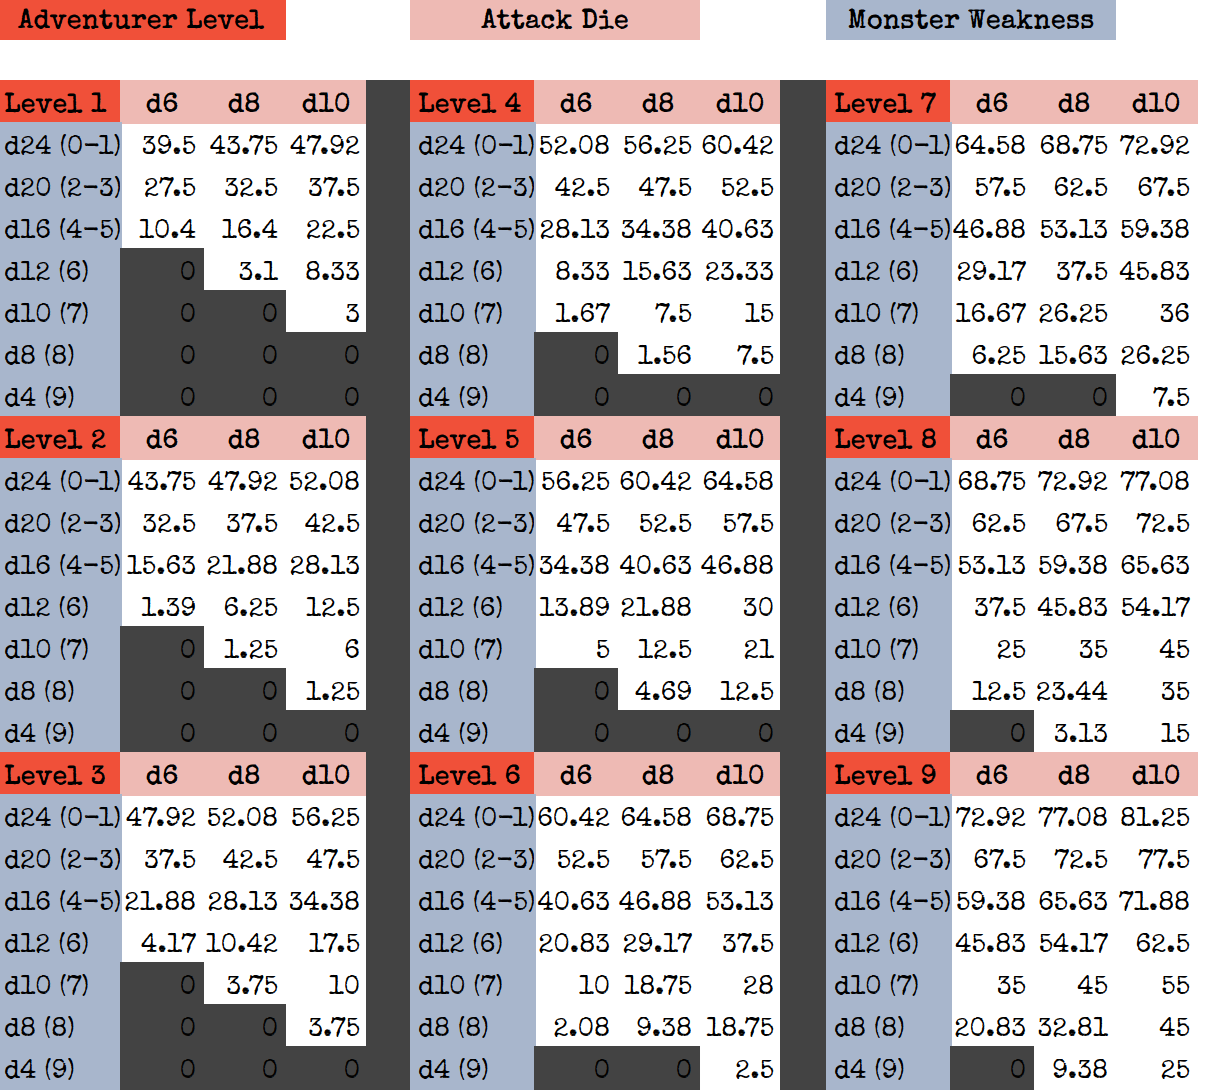
\includegraphics[width=.9\linewidth,keepaspectratio=true]{appendices/AttackOdds}
    \end{center}

\mysubsection{Adventurer Grit (Basic)}{dice-adventurer-grit}

\mytable{Y Y Y Y} {
    \thead{Adventurer Level} & \thead{Mean} & \thead{Min} & \thead{Max} \\
}{
    2 & 6 & 3 & 9 \\
    3 & 7.5 & 3 & 12 \\
    4 & 10.5 & 3 & 18 \\
    5 & 10.5 & 3 & 18 \\
    6 & 10.5 & 3 & 18 \\
    7 & 13.5 & 3 & 24 \\
    8 & 13.5 & 3 & 24 \\
    9 & 13.5 & 3 & 24 \\
   \mybold{Total} & \mybold{85.5} & \mybold{24} & \mybold{147} \\
}

  \newpage
  \mysection{Appendix D: The Small Gods}{appendix-d}

\begin{multicols*}{2}

These are the seven most numerous Small Gods worshiped on Acheron beneath each \mylink{Paradigm}{faith-paradigm}.  This isn't even close to a complete list, for the Small Gods are as numerous as the stars ...


\mysubsection{Civilized Small Gods}{civilized-small-gods}

\myimage{appendices/CivilizedParadigm}

\GOD[Name=Balder,GodOf=Seraph of Beauty and Gems,Holy={a silver mirror}]

\GOD[Name=Gomorrah,GodOf=Archfiend of Cities,Holy={a single iron nail, often driven into the hand or wrist}]

\GOD[Name=Minerva,GodOf=Archon of Trade and Commerce,Holy={a knotted string, hung from the belt, useful for counting (like an abacus)}]

\GOD[Name=Nimlurun,GodOf=Fiend of Filth and Pollution,Holy={an iron vial of sewer water}]

\GOD[Name=Ninkasi,GodOf={Seraph of Art, Music and Fermentation},Holy={an iron amulet hung from a necklace in the exact size and shape of a modern bottle opener}]

\GOD[Name=Ptah,GodOf=God of Builders,Holy={an amulet in the shape of an ankh}]

\GOD[Name=Vulcan,GodOf=Seraph of the Forge,Holy={a small crude homonculous, hammered from iron}]


\mysubsection{Cthonic Small Gods}{cthonic-small-gods}

\GOD[Name=Arioch,GodOf=Fiend of Murder and Betrayal,Holy={a silver coin with a face on each side}]

\GOD[Name=Erebus,GodOf=Lord of Shadows,Holy={a piece of black gauze covering the mouth}]

\GOD[Name=Loki,GodOf=King of Thieves,Holy={an image of two snakes, circling one another to form an 'S' shape, and biting the tail of the other}]

\myimage{appendices/CthonicParadigm}

\GOD[Name=Nyx,GodOf=Cousin of Death,Holy={a black lace shroud}]

\GOD[Name=Shezmu,GodOf=Prince of Blood,Holy={a vial of blood other than your own (preferably the blood of the one who indoctrinated you into the faith)}]

\GOD[Name=Tik'tak'mennippi,GodOf=Prince of the Drowned,Holy={a necklace made from crab's claws and nautical rope, tied in elaborate knots}]

\GOD[Name=The Yellow King,GodOf=Fiend of Illusion and Disguises,Holy={a yellow cowl and mask}]



\mysubsection{Cunning Small Gods}{cunning-small-gods}

\GOD[Name=Cthulhu,GodOf=Arbiter of Mysteries and Riddles,Holy={A piece of jewelry depicting an octopus}]

\GOD[Name=Hecate,GodOf=Archfiend of Wizardry,Holy={a Grimoire}]

\GOD[Name=Iktomi,GodOf=God of Tricksters,Holy={a small puppet, worn from the belt or neck}]


\myimage{appendices/CunningParadigm}

\GOD[Name=M{\AccentI}mir,GodOf=God of Runes,Holy={a necklace of tiles inscribed with runes}]

\GOD[Name=The Grey Men,GodOf=Archons of Diplomacy,Holy={a choker of dove feathers}]

\GOD[Name=The Muses,GodOf=Gods of Inspiration,Holy={a nine-pointed star, worn as an amulet or inscribed on a headband}]

\GOD[Name=Thoth,GodOf=God of Knowledge,Holy={a small book of scripture}]

\myimage{appendices/EmpyreanParadigm}


\mysubsection{Empyrean Small Gods}{empyrean-small-gods}

\GOD[Name=Asura,GodOf=Seraph of Sunlight,Holy={polished mirrors or brass, hung from the neck or belt}]

\GOD[Name=Empress Wa,GodOf=God of the Heavens,Holy={a jade diadem}]

\GOD[Name=Raiden,GodOf=Lord of Lightning,Holy={two iron bracers with lightning bolts etched on them}]

\GOD[Name=Raimonds Mountainhand,GodOf=Seraph of the Mountaintops,Holy={3 iron spikes in the shape of icicles or teeth, hung from the neck}]

\GOD[Name=Shul,GodOf=Seraph of Moonlight,Holy={3 pearl earrings, hung from either ear}]

\GOD[Name=Tiamat,GodOf=Fiendish Prince of Tempests,Holy={a five pointed star, worn from a necklace}]

\GOD[Name=Tlaloc,GodOf=Archon of the Rains,Holy={a wreath of ferns and mosses}]



\mysubsection{Errant Small Gods}{errant-small-gods}

\GOD[Name=Balo,GodOf=Archon of Games and Contests,Holy={a leather bag of bone dice, hung from the neck or belt}]

\GOD[Name=Gilgamesh,GodOf=Lord of Strength and Valor,Holy={a pair of bull's horns, hung from the neck or worn as a helmet}]

\GOD[Name=Izzek Unchained,GodOf=Seraph of Suffering and Freedom,Holy={a broken pair of manacles}]

\GOD[Name=Kismet,GodOf=Arbiter of Journeys,Holy={a carved walking stick}]

\GOD[Name=Odysseus,GodOf=God of Homecomings,Holy={an iron wheel hanging from a bowstring necklace}]

\GOD[Name=St. Ant{\AccentO}nios,GodOf=Lord of Lost Treasures,Holy={a coin (gold is best) with a hole through the center, worn on a chain}]

\GOD[Name=Xbalanque and Hunahpu,GodOf=Twin Gods of Trials,Holy={two ears of dried corn (hung from a belt, around the neck, etc.)}]



\myimage{appendices/ErrantParadigm}

\mysubsection{Heathen Small Gods}{heathen-small-gods}

\GOD[Name=Brigid,GodOf=Seraph of Hearth and Gardens,Holy={a shillelagh}]

\GOD[Name=Cernunnos,GodOf=Archon of the Hunt,Holy={a tine of the antler of a game animal}]

\GOD[Name=The Green Man,GodOf=Lord of the Wood,Holy={a crown of ivy or holly}]

\GOD[Name=Ishtar,GodOf=Lady of Fertility and Agriculture,Holy={an eight pointed star, usually worn as an amulet}]

\GOD[Name=Lirazel,GodOf=Lady of the Glade,Holy={a vial of clear water}]

\begin{center}
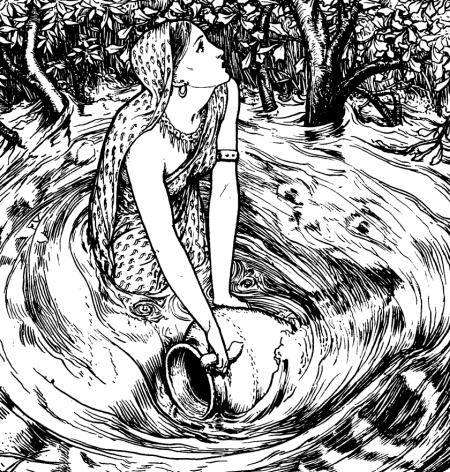
\includegraphics[scale=.4]{appendices/HeathenParadigm}
\end{center}


\GOD[Name=Malachi,GodOf=Minder of Songs{,} Poetry{,} and Ancestors,Holy={a small musical instrument}]

\GOD[Name=Pilzesser,GodOf=Seraph of Hallucinogenic Plants and Fungi,Holy={a symbol of a pyramid with an eye at the top, and the letters "FNORD" along its base.  Worn on a necklace or headband}]


\mysubsection{J{\UmlautO}tnar Small Gods}{jotnar-small-gods}

\GOD[Name=Cr{\UmlautO}m,GodOf=Arbiter of Honorable Death,Holy={the devotee must name one of their weapons; this weapon will be used as their holy symbol}]

\GOD[Name=C{\AccentU} Chulainn,GodOf=God of the Battle Frenzy,Holy={a headdress of raven or crow feathers}]


\GOD[Name=Justicia,GodOf=Seraph of Vengeance,Holy={An image or symbol of something the Devotee wants vengeance against}]

\GOD[Name=The Morning Star,GodOf=Fiendish Prince of Fire,Holy={a red stone (agate, garnet, carnelian, red cinnabar, etc) worn on a choker.}]


\GOD[Name=Odin,GodOf=Archon of Strategy and Combat,Holy={3 interlocking triangles, worn as a necklace from a chain}]

\GOD[Name=Xenophon,GodOf=Archon of Mercenaries and Assassins,Holy={3 rusted iron coins, sewn or welded to a bracelet on the dominant hand}]



\GOD[Name=Ymir,GodOf=Archon of Ice and Snow,Holy={quartz stones affixed to a pair of leather or iron bracers}]


\mysubsection{Monstrous Small Gods}{monstrous-small-gods}

\GOD[Name=Ariadne,GodOf=Princess of Spiders,Holy={a gossamer veil}]

\GOD[Name=Bast,GodOf=Archon of Cats,Holy={a small bell without a clapper, worn on a choker}]


\GOD[Name=God of Rats,GodOf=Prince of Rats and Vermin,Holy={a mouse-skin glove worn on the dominant hand}]


\GOD[Name=J{\UmlautO}rmungandr,GodOf=Duke of Serpents,Holy={snakeskin bracers}]


\GOD[Name=Ptah-Ungurath,GodOf=Archfiend of Monsters,Holy={an amulet in the shape of an upside-down ankh}]

\begin{center}
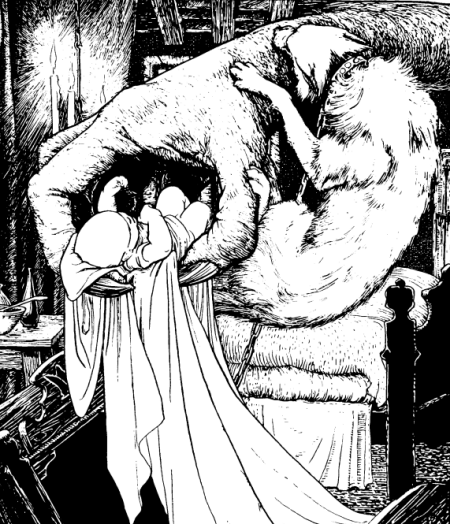
\includegraphics[scale=.35]{appendices/MonstrousParadigm}
\end{center}



\GOD[Name=Tengu,GodOf=Archon of Birds,Holy={a short cloak of feathers}]

\GOD[Name=Whort,GodOf=Prince of Toads,Holy={3 desiccated frogs, worn from the belt or neck}]


\mysubsection{Righteous Small Gods}{righteous-small-gods}

\GOD[Name=Anubis,GodOf=Fiend of Judgment and Punishment,Holy={a set of scales hung from a chain}]

\GOD[Name=Bahamut,GodOf=Lord of Truth and Light,Holy={an iron or silver circlet, embossed with an arrow pointing upwards}]

\GOD[Name=Chrontics,GodOf=Lord of Time,Holy={an amulet (silver preferred) embossed with a hammered hourglass}]

\GOD[Name=Marduk,GodOf=God of Law ,Holy={an unblinking eye worn on a linen headband}]

\GOD[Name=Mitra,GodOf=Seraph of Obedience and Protection,Holy={an iron thorn, coincidentally in the shape of a modern bullet, suspended from a chain around the neck}]

\GOD[Name=T{\AccentI}r,GodOf=Seraph of Order,Holy={an iron sleeve worn over the non-dominant hand (the hand is unable to hold anything)}]

\GOD[Name=V{\AccentA}r,GodOf=Seraph of Oaths and Agreements,Holy={a crystal vial containing the blood and spit of two Mortals who have struck a deal with one another}]

\begin{center}
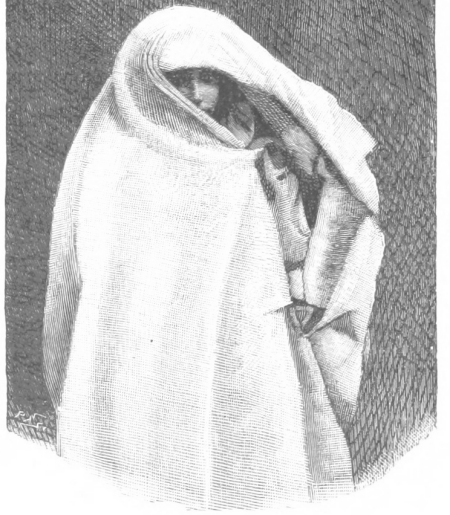
\includegraphics[scale=.3]{appendices/RighteousParadigm}
\end{center}

\mysubsection{Ruinous Small Gods}{ruinous-small-gods}

\GOD[Name=Erinys,GodOf=Archfiend of Curses,Holy={a severed hand hung from the neck or belt}]


\GOD[Name=Fortuna,GodOf=Seraph of Luck,Holy={a deck of cards}]


\cbreak

\GOD[Name=Nergal,GodOf=God of Dooms,Holy={an iron mask}]

\GOD[Name=The Wendigo,GodOf=God of Hunger,Holy={a necklace of teeth}]

\myimage{appendices/RuinousParadigm}

\GOD[Name=The Morrigan,GodOf=Archon(s) of Fate,Holy={a triangle whose points extend into counterclockwise swirls, usually worn on a headband or scarf}]

\GOD[Name=Xibalba,GodOf=Fiendish Prince of Fear,Holy={a white cowl and blank mask}]

\GOD[Name=Zuul,GodOf=Archfiend of Destruction,Holy={a ceramic circle broken in half, worn on the belt or a necklace}]


\end{multicols*}

\mysubsection{Liturgical Guide}{table-liturgical-guide}

\mytable{X X X}{
	 \thead{Paradigm} &\thead{Liturgy} &\thead{Formulary} \\ 
}{
	 	 Civilized & \mylink{Armor of the Gods}{arcana-mystery-armor-of-the-gods} & Ablution \\ 
	 	 Civilized & \mylink{Army of the Pharoahs}{arcana-mystery-army-pharoahs} & Lorespell \\ 
	 	 Civilized & \mylink{Bastion}{arcana-mystery-aura-protection} & Orison \\ 
	 	 Civilized & \mylink{Blessed Brew}{arcana-mystery-blessed-brew} & Ablution \\ 
	 	 Civilized & \mylink{Hone}{arcana-mystery-hone} & Hymn \\ 
	 	 Civilized & \mylink{Indomitable Mail}{arcana-mystery-instantaneous-repair} & Hymn \\ 
	 	 Civilized & \mylink{Lay Assistance}{arcana-mystery-lay-assistance} & Lorespell \\ 
	 	 Civilized & \mylink{Pestilential Breath}{arcana-mystery-pestilential-breath} & Orison \\ 
	 	 Cthonic & \mylink{Abyssal Trident}{arcana-mystery-abyssal-trident} & Hymn \\ 
	 	 Cthonic & \mylink{Davy Jones's Locker}{arcana-mystery-davy-joness-locker} & Ablution \\ 
	 	 Cthonic & \mylink{Fade}{arcana-mystery-fade} & Orison \\ 
	 	 Cthonic & \mylink{Mermaid's Breath}{arcana-mystery-mermaids-breath} & Lorespell \\ 
	 	 Cthonic & \mylink{Misericorde}{arcana-mystery-misericorde} & Hymn \\ 
	 	 Cthonic & \mylink{Sanguine Remedy}{arcana-mystery-sanguine-remedy} & Ablution \\ 
	 	 Cthonic & \mylink{Sound the Deeps}{arcana-mystery-sound-the-deeps} & Lorespell \\ 
	 	 Cthonic & \mylink{Wyrmbreath}{arcana-mystery-wyrmbreath} & Orison \\ 
	 	 Cunning & \mylink{Divine Inspiration}{arcana-mystery-divine-inspiration} & Orison \\ 
	 	 Cunning & \mylink{Doppelg{\UmlautA}nger}{arcana-mystery-doppelganger} & Ablution \\ 
	 	 Cunning & \mylink{Hecates' Blessing}{arcana-mystery-hecates-blessing} & Hymn \\ 
	 	 Cunning & \mylink{Memory Lane}{arcana-mystery-memory-lane} & Lorespell \\ 
	 	 Cunning & \mylink{Mirage}{arcana-mystery-mirage} & Lorespell \\ 
	 	 Cunning & \mylink{Mirror Image}{arcana-mystery-mirror-image} & Ablution \\ 
	 	 Cunning & \mylink{Spook}{arcana-mystery-spook} & Orison \\ 
	 	 Cunning & \mylink{Vulpine Wisdom}{arcana-mystery-vulpine-wisdom} & Hymn \\ 
	 	 Empyrean & \mylink{Children of Shul}{arcana-mystery-children-of-shul} & Ablution \\ 
	 	 Empyrean & \mylink{Dervish}{arcana-mystery-dervish} & Orison \\ 
	 	 Empyrean & \mylink{Lightning}{arcana-mystery-lightning} & Orison \\ 
	 	 Empyrean & \mylink{Mountainhands}{arcana-mystery-mountainhands} & Hymn \\ 
	 	 Empyrean & \mylink{Noontide}{arcana-mystery-noontide} & Lorespell \\ 
	 	 Empyrean & \mylink{Sirocco}{arcana-mystery-sirocco} & Hymn \\ 
	 	 Empyrean & \mylink{Welkin's Gaze}{arcana-mystery-welkin-gaze} & Ablution \\ 
	 	 Errant & \mylink{Capture Wind}{arcana-mystery-capture-wind} & Lorespell \\ 
	 	 Errant & \mylink{Corsair's Blade}{arcana-mystery-corsairs-blade} & Ablution \\ 
	 	 Errant & \mylink{Great Strength}{arcana-mystery-great-strength} & Hymn \\ 
	 	 Errant & \mylink{Hand of God}{arcana-mystery-hand-of-god} & Orison \\ 
	 	 Errant & \mylink{Lady Luck}{arcana-lady-luck} & Ablution \\ 
	 	 Errant & \mylink{On Your Feet}{arcana-mystery-on-your-feet} & Orison \\ 
	 	 Errant & \mylink{Shatter Bonds}{arcana-mystery-shatter-bonds} & Lorespell \\ 
	 	 Errant & \mylink{Vaulting Step}{arcana-mystery-vaulting-step} & Hymn \\ 
}

\newpage

\mytable{X X X}{
	 \thead{Paradigm} &\thead{Liturgy} &\thead{Formulary} \\ 
}{
	 	 Heathen & \mylink{Barkskin}{arcana-mystery-barkskin} & Ablution \\ 
	 	 Heathen & \mylink{Clearwater}{arcana-mystery-clearwater} & Lorespell \\ 
	 	 Heathen & \mylink{Elemental Spray}{arcana-mystery-elemental-spray} & Orison \\ 
	 	 Heathen & \mylink{Hearthfire}{arcana-mystery-hearthfire} & Lorespell \\ 
	 	 Heathen & \mylink{Rainburst}{arcana-mystery-rainburst} & Lorespell \\ 
	 	 Heathen & \mylink{Rootshield}{arcana-mystery-rootshield} & Hymn \\ 
	 	 Heathen & \mylink{Sacred Smoke}{arcana-mystery-sacred-smoke} & Ablution \\ 
	 	 Heathen & \mylink{Sporous Vapor}{arcana-mystery-sporous-vapor} & Orison \\ 
	 	 Heathen & \mylink{Whip of Thorns}{arcana-mystery-whip-of-thorns} & Hymn \\ 
	 	 J{\UmlautO}tnar & \mylink{Dirge}{arcana-mystery-dirge} & Lorespell \\ 
	 	 J{\UmlautO}tnar & \mylink{Giantform}{arcana-mystery-giantform} & Lorespell \\ 
	 	 J{\UmlautO}tnar & \mylink{Incinerate}{arcana-mystery-incinerate} & Ablution \\ 
	 	 J{\UmlautO}tnar & \mylink{Prayer for the Dying}{arcana-mystery-prayer-dying} & Orison \\ 
	 	 J{\UmlautO}tnar & \mylink{Preserve}{arcana-mystery-preserve} & Ablution \\ 
	 	 J{\UmlautO}tnar & \mylink{Ray of Fire}{arcana-mystery-ray-of-fire} & Orison \\ 
	 	 J{\UmlautO}tnar & \mylink{Trollblood}{arcana-mystery-trollblood} & Hymn \\ 
	 	 J{\UmlautO}tnar & \mylink{Witness Me}{arcana-mystery-witness-me} & Hymn \\ 
	 	 Monstrous & \mylink{Feline Ease}{arcana-mystery-feline-ease} & Orison \\ 
	 	 Monstrous & \mylink{Gory Locks}{arcana-mystery-gory-locks} & Ablution \\ 
	 	 Monstrous & \mylink{Monstrous Aspect}{arcana-mystery-monstrous-aspect} & Hymn \\ 
	 	 Monstrous & \mylink{Poison Spittle}{arcana-mystery-poison-spittle} & Orison \\ 
	 	 Monstrous & \mylink{Pummeling Hands}{arcana-mystery-pummeling-hands} & Hymn \\ 
	 	 Monstrous & \mylink{Slimeform}{arcana-mystery-slimeform} & Ablution \\ 
	 	 Monstrous & \mylink{Tasty}{arcana-mystery-tasty} & Lorespell \\ 
	 	 Monstrous & \mylink{Tattered Robe}{arcana-mystery-tattered-robe} & Lorespell \\ 
	 	 Righteous & \mylink{Blessed Blade}{arcana-mystery-blessed-blade} & Hymn \\ 
	 	 Righteous & \mylink{Crusader's Helm}{arcana-mystery-crusaders-helm} & Ablution \\ 
	 	 Righteous & \mylink{Eye of Flame}{arcana-mystery-eye-of-flame} & Hymn \\ 
	 	 Righteous & \mylink{Fortifying Blaze}{arcana-mystery-fortifying-blaze} & Lorespell \\ 
	 	 Righteous & \mylink{Resonating Command}{arcana-mystery-resonating-command} & Orison \\ 
	 	 Righteous & \mylink{Revered Aegis}{arcana-mystery-revered-aegis} & Ablution \\ 
	 	 Righteous & \mylink{Satanic Verses}{arcana-mystery-satanic-verses} & Lorespell \\ 
	 	 Righteous & \mylink{Scourge of Chaos}{arcana-mystery-scourge-of-chaos} & Orison \\ 
	 	 Ruinous & \mylink{Gaze of the Void}{arcana-mystery-gaze-of-the-void} & Orison \\ 
	 	 Ruinous & \mylink{Hand of Fate}{arcana-mystery-hand-of-fate} & Ablution \\ 
	 	 Ruinous & \mylink{Lucky Throw}{arcana-mystery-lucky-throw} & Hymn \\ 
	 	 Ruinous & \mylink{Plague}{arcana-mystery-plague} & Lorespell \\ 
	 	 Ruinous & \mylink{Rending Strike}{arcana-mystery-rending-strike} & Hymn \\ 
	 	 Ruinous & \mylink{Sceptre of Ruin}{arcana-mystery-lucky-day} & Ablution \\ 
	 	 Ruinous & \mylink{Vile Hunger}{arcana-mystery-vile-hunger} & Orison \\ 
	 	 Ruinous & \mylink{Wall of Gloom}{arcana-mystery-wall-of-gloom} & Lorespell \\ 
}

  \newpage
  \mysection{Appendix E: The Virtues}{appendix-e}


\mysubsection{Knave Virtues}{appendix-e-knave-virtues}

{\footnotesize{
  \mytable{X X X X} {
    \thead{Greenhorn (Level 1)} & \thead{Daredevil (Level 2+)} & \thead{Heroic (Level 4+)} & \thead{Legendary (Level 7+)} \\
  } {
        \mylink{Charms}{knave-virtue-charms} & \mylink{Beginner's Luck}{adv-knave-virtue-beginners-luck} & \mylink{Kismet}{adv-knave-virtue-kismet} & \mylink{Astonishing Luck}{adv-knave-virtue-astonishing-luck} \\ 
        \mylink{Deadeye}{knave-virtue-deadeye} & \mylink{Charms}{adv-knave-virtue-charms} & \mylink{Left-Hand Path (Sharper)}{adv-knave-virtue-left-hand-path-sharper} & \mylink{Guildmaster}{adv-knave-virtue-guildmaster} \\ 
        \mylink{Guilded}{knave-virtue-guilded} & \mylink{Deadeye}{adv-knave-virtue-deadeye} & \mylink{Personality}{adv-knave-virtue-personality} & \mylink{Kismet}{adv-knave-virtue-kismet} \\ 
        \mylink{Hard to Kill}{knave-virtue-hard-to-kill} & \mylink{Kismet}{adv-knave-virtue-kismet} & \mylink{Precepts of Blight}{adv-knave-virtue-blight} & \mylink{Left-Hand Path (Master)}{adv-knave-virtue-left-hand-path-master} \\ 
        \mylink{Inked}{knave-virtue-inked} & \mylink{L.Hand Path (Apprentice)}{adv-knave-virtue-left-hand-path-apprentice} & \mylink{Precepts of Blood}{adv-knave-virtue-blood} & \mylink{Personality}{adv-knave-virtue-personality} \\ 
        \mylink{Medicine}{knave-virtue-medicine} & \mylink{Left-Hand Path (Footpad)}{adv-knave-virtue-left-hand-path-footpad} & \mylink{Precepts of Celerity}{adv-knave-virtue-celerity} & \mylink{Saves}{adv-knave-virtue-saves} \\ 
        \mylink{Mummy's Curse}{knave-virtue-mummys-curse} & \mylink{Medicine}{adv-knave-virtue-medicine} & \mylink{Precepts of Wizardry}{adv-knave-virtue-blood-wizardry} & \mylink{Surprise Motherfucker!}{adv-knave-virtue-surprise-motherfucker} \\ 
        \mylink{Sacraments}{knave-virtue-vulgate-sacraments} & \mylink{Mummy's Curse}{adv-knave-virtue-mummys-curse} & \mylink{Saves}{adv-knave-virtue-saves} & \mylink{The Plan}{adv-knave-virtue-the-plan} \\ 
        \mylink{Whispers of Anne Bonny}{knave-virtue-anne-bonny} & \mylink{Personality}{adv-knave-virtue-personality} & \mylink{Uncanny Luck}{adv-knave-virtue-uncanny-luck} & - \\ 
        \mylink{Whispers of Br'er Rabbit}{knave-virtue-brer-rabbit} & \mylink{Sacraments}{adv-knave-virtue-sacraments} & \mylink{Unlabeled Package}{adv-knave-virtue-unlabeled-package} & - \\ 
        \mylink{Whispers of Sun Wukong}{knave-virtue-sun-wukong} & \mylink{Saves}{adv-knave-virtue-saves} & - &- \\ 
        \mylink{Whispers of The Bride}{knave-virtue-the-bride} & \mylink{Slippery}{adv-knave-virtue-slippery} & - &- \\
}}}


\mysubsection{Mystic Virtues}{appendix-e-mystic-virtues}

{\footnotesize{
  \mytable{X X X X} {
    \thead{Greenhorn (Level 1)} & \thead{Daredevil (Level 2+)} & \thead{Heroic (Level 4+)} & \thead{Legendary (Level 7+)} \\
  } {
        \mylink{Bruja}{mystic-virtue-bruja} & \mylink{Charms}{adv-mystic-charms} & \mylink{Cloister}{adv-mystic-cloister} & \mylink{Charmed Circle}{adv-mystic-charmed-circle} \\ 
        \mylink{Charms}{mystic-virtue-vulgate-charms} & \mylink{Cunning Folk}{adv-mystic-cunning-folk} & \mylink{Feyness}{adv-mystic-feyness} & \mylink{Fishers of Men}{adv-mystic-fishers-of-men} \\ 
        \mylink{Cunning Folk}{mystic-virtue-cunning-folk} & \mylink{Devotion}{adv-mystic-devotion} & \mylink{Kismet}{adv-mystic-kismet} & \mylink{Kismet}{adv-mystic-kismet} \\ 
        \mylink{Hand of God}{mystic-virtue-hand-of-god} & \mylink{Kismet}{adv-mystic-kismet}  & \mylink{Liturgies: Apostles}{adv-mystic-liturgy-apostles} & \mylink{Liturgies: Saints}{adv-mystic-liturgy-saints} \\ 
        \mylink{Holy Warrior}{mystic-virtue-holy-warrior} & \mylink{Liturgies: Clerics}{adv-mystic-liturgy-clerics} & \mylink{Master of Puppets}{adv-mystic-master-of-puppets} & \mylink{Necromancer}{adv-mystic-necromancer} \\ 
        \mylink{Initiate}{mystic-virtue-initiate} & \mylink{Liturgies: Novitiates}{adv-mystic-liturgy-novitiates} & \mylink{Personality}{adv-mystic-personality} & \mylink{Norn's Shears}{adv-mystic-norns-shears} \\ 
        \mylink{Itinerant}{mystic-virtue-itinerant} & \mylink{Medicine}{adv-mystic-medicine} & \mylink{Saves}{adv-mystic-saves} & \mylink{Personality}{adv-mystic-personality} \\ 
        \mylink{Medicine}{mystic-virtue-vulgate-medicine} & \mylink{Mombo}{adv-mystic-mombo} & \mylink{Tongues of Fire}{adv-mystic-tongues-of-fire} & \mylink{Saves}{adv-mystic-saves} \\ 
        \mylink{Miracle Worker}{mystic-virtue-miracle-worker} & \mylink{Personality}{adv-mystic-personality} & \mylink{Uncanny}{adv-mystic-uncanny}  & - \\ 
        \mylink{Mombo}{mystic-virtue-mombo} & \mylink{Sacraments}{adv-mystic-sacraments} & \mylink{Witch}{adv-mystic-witch}  & - \\ 
        \mylink{Sacraments}{mystic-virtue-vulgate-sacraments} & \mylink{Saves}{adv-mystic-saves} & -  &- \\ 
        \mylink{Sacred Flesh}{mystic-virtue-sacred-flesh} & \mylink{Wisdom}{adv-mystic-wisdom} & - &- \\ 

}}}



\mysubsection{Philosopher Virtues}{appendix-e-philosopher-virtues}

{\footnotesize{
  \mytable{X X X X} {
    \thead{Greenhorn (Level 1)} & \thead{Daredevil (Level 2+)} & \thead{Heroic (Level 4+)} & \thead{Legendary (Level 7+)} \\
  } {
        \mylink{Bagman}{philosopher-virtue-bagman} & \mylink{Charms}{adv-philosopher-charms} & \mylink{Anarchist}{adv-philosopher-anarchist} & \mylink{Kallisti}{adv-philosopher-kallisti} \\ 
        \mylink{Charms}{philosopher-virtue-charms} & \mylink{Chymist}{adv-philosopher-chymist} & \mylink{Conduit of Blood}{adv-philosopher-conduit-blood} & \mylink{Kismet}{adv-philosopher-kismet} \\ 
        \mylink{Chymist}{philosopher-virtue-chymist} & \mylink{Discordian}{adv-philosopher-discordian} & \mylink{Doctor}{adv-philosopher-doctor} & \mylink{Maestro}{adv-philosopher-maestro} \\ 
        \mylink{College}{philosopher-virtue-college} & \mylink{Kismet}{adv-philosopher-kismet} & \mylink{Esteemed}{adv-philosopher-esteemed} & \mylink{Patron}{adv-philosopher-patron} \\ 
        \mylink{Discordian}{philosopher-virtue-discordian} & \mylink{Medicine}{adv-philosopher-medicine} & \mylink{Kismet}{adv-philosopher-kismet} & \mylink{Personality}{adv-philosopher-personality} \\ 
        \mylink{Invoker}{philosopher-virtue-invoker} & \mylink{Personality}{adv-philosopher-personality} & \mylink{Knowledge is Power}{adv-philosopher-knowledge-power} & \mylink{Saves}{adv-philosopher-saves} \\ 
        \mylink{Medicine}{philosopher-virtue-medicine} & \mylink{Professor}{adv-philosopher-professor} & \mylink{Personality}{adv-philosopher-personality} & \mylink{Staff Magic: Archmage}{adv-philosopher-staff-archmage} \\ 
        \mylink{Praxis}{philosopher-virtue-praxis} & \mylink{Sacraments}{adv-philosopher-sacraments} & \mylink{Saves}{adv-philosopher-saves} & \mylink{Tutor}{adv-philosopher-tutor} \\ 
        \mylink{Sacraments}{philosopher-virtue-vulgate-sacraments} & \mylink{Saves}{adv-philosopher-saves} & \mylink{Staff Magic: Warlock}{adv-philosopher-staff-warlock} & - \\ 
        \mylink{Scribe}{philosopher-virtue-scribe} & \mylink{Scribe}{adv-philosopher-scribe} & \mylink{Well Read}{adv-philosopher-well-read}  & - \\ 
        \mylink{Sorcerer}{aphilosopher-virtue-sorcerer} & \mylink{Sorcerer}{adv-philosopher-sorcerer} & - &- \\ 
        \mylink{Staff Magic: Novice}{philosopher-virtue-staff-magic} & \mylink{Staff Magic: Novice}{adv-philosopher-staff-novice} & - &- \\ 
}}}


\mysubsection{Sellsword Virtues}{appendix-e-sellsword-virtues}

{\footnotesize{
  \mytable{X X X X} {
    \thead{Greenhorn (Level 1)} & \thead{Daredevil (Level 2+)} & \thead{Heroic (Level 4+)} & \thead{Legendary (Level 7+)} \\
  } {
        \mylink{Blademaster}{sellsword-virtue-blademaster} & \mylink{Blademaster}{adv-sellsword-blademaster} & \mylink{Berserker}{adv-sellsword-berserker} & \mylink{Captain}{adv-sellsword-captain} \\ 
        \mylink{Charms}{sellsword-virtue-vulgate-charms} & \mylink{Charms}{adv-sellsword-charms} & \mylink{Boxer}{adv-sellsword-boxer} & \mylink{Death Dancer}{adv-sellsword-death-dancer} \\ 
        \mylink{Deadly}{sellsword-virtue-deadly} & \mylink{Deadly}{adv-sellsword-deadly} & \mylink{Command}{adv-sellsword-command} & \mylink{Inspiration}{adv-sellsword-inspiration} \\ 
        \mylink{Harder Than a Coffin Nail}{sellsword-virtue-coffin-nail} & \mylink{Expertise}{adv-sellsword-expertise} & \mylink{Kismet}{adv-sellsword-kismet} & \mylink{Kismet}{adv-sellsword-kismet} \\ 
        \mylink{Hunter}{sellsword-virtue-hunter} & \mylink{Kismet}{adv-sellsword-kismet} & \mylink{Mastery}{adv-sellsword-mastery} & \mylink{Mortal Blow}{adv-sellsword-mortal-blow} \\ 
        \mylink{Medicine}{sellsword-virtue-vulgate-medicine} & \mylink{Medicine}{adv-sellsword-medicine} & \mylink{Personality}{adv-sellsword-personality} & \mylink{Personality}{adv-sellsword-personality} \\ 
        \mylink{My Father's Sword}{sellsword-virtue-fathers-sword} & \mylink{Personality}{adv-sellsword-personality} & \mylink{Saves}{adv-sellsword-saves} & \mylink{Righteous Blade}{adv-sellsword-righteous-blade} \\ 
        \mylink{Sacraments}{sellsword-virtue-vulgate-sacraments} & \mylink{Sacraments}{adv-sellsword-sacraments} & \mylink{Survivor}{adv-sellsword-survivor} & \mylink{Saves}{adv-sellsword-saves} \\ 
        \mylink{Second Skin}{sellsword-virtue-second-skin} & \mylink{Saves}{adv-sellsword-saves} & \mylink{Sword Saint}{adv-sellsword-sword-saint} & - \\ 
        \mylink{Three Kills Per Stroke}{sellsword-virtue-three-kills} & \mylink{Sixth Sense}{adv-sellsword-sixth-sense} & \mylink{Valor}{adv-sellsword-valor} & - \\ 
        \mylink{Veteran}{sellsword-virtue-veteran} & \mylink{Three Kills Per Stroke}{adv-sellsword-three-kills} & - &- \\ 
        \mylink{Won't Stay Down}{sellsword-virtue-stay-down} & \mylink{Warder}{adv-sellsword-warder} & - &- \\
}}}


\mysubsection{Murk Virtues}{appendix-e-murk-virtues}

{\footnotesize{
  \mytable{X X X X} {
    \thead{Greenhorn (Level 1)} & \thead{Daredevil (Level 2+)} & \thead{Heroic (Level 4+)} & \thead{Legendary (Level 7+)} \\
  } {
        \mylink{Cat's Eyes}{murk-virtue-cats-eyes} & \mylink{Apprentice of the Bride}{adv-murk-bride} & \mylink{Footpad of the Bride}{adv-murk-footpad} & \mylink{Kismet}{adv-murk-kismet} \\
        \mylink{Emancipated}{murk-emancipated} & \mylink{Charms}{adv-murk-charms} & \mylink{Invisibility}{adv-murk-invisibility} & \mylink{Loner}{adv-murk-loner} \\
        \mylink{Fate's Hand}{murk-virtue-fates-hand} & \mylink{Ghost}{adv-murk-ghost} & \mylink{Kismet}{adv-murk-kismet} & \mylink{Personality}{adv-murk-personality} \\
        \mylink{Killer}{murk-virtue-killer} & \mylink{Kismet}{adv-murk-kismet} & \mylink{Personality}{adv-murk-personality} & \mylink{Saves}{adv-murk-saves} \\
        \mylink{Metal Empathy}{murk-virtue-metal-empathy} & \mylink{Personality}{adv-murk-personality} & \mylink{Saves}{adv-murk-saves} & \mylink{Sharper of the Bride}{adv-murk-sharper} \\
        \mylink{Silent Speech}{murk-virtue-silent-speech} & \mylink{Saves}{adv-murk-saves} & \mylink{Self-Reliant}{adv-murk-self-reliant} & \mylink{Stonewalker}{adv-murk-stonewalker} \\
        \mylink{Undreamt}{murk-virtue-undreamt} & \mylink{Self-Sufficient}{adv-murk-self-sufficient} & \mylink{Shadowblade}{adv-murk-shadowblade} & - \\
        - & \mylink{Stonespeaker}{adv-murk-stonespeaker} & \mylink{Stoneshaper}{adv-murk-stone-shaper} & - \\
        - & \mylink{Will to Live}{adv-murk-will-to-live} & - & -\\
        - & \mylink{You and Me}{adv-murk-you-and-me} & - & - \\
}}}

\mysubsection{Pooka Virtues}{appendix-e-pooka-virtues}

{\footnotesize{
  \mytable{X X X X} {
    \thead{Greenhorn (Level 1)} & \thead{Daredevil (Level 2+)} & \thead{Heroic (Level 4+)} & \thead{Legendary (Level 7+)} \\
  } {

        \mylink{Apotropaic}{pooka-virtue-apotropaic} & \mylink{Apprentice of the Rabbit}{adv-pooka-apprentice-rabbit} & \mylink{Epic Songs}{adv-pooka-epic-songs} & \mylink{Kismet}{adv-pooka-kismet} \\
        \mylink{Bro, Hit This}{pooka-virtue-hit-this} & \mylink{Calling in the Markers}{adv-pooka-markers} & \mylink{Fast Metabolism}{adv-pooka-fast-metabolism} & \mylink{Martyrdom}{adv-pooka-martyrdom} \\
        \mylink{Curious}{pooka-curious} & \mylink{Fortunate}{adv-pooka-fortunate} & \mylink{Footpad of the Rabbit}{adv-pooka-footpad-rabbit} & \mylink{Personality}{advancement-pooka-personality} \\
        \mylink{Hype Man}{pooka-virtue-hype-man} & \mylink{Healing Wax}{adv-pooka-healing} & \mylink{Kismet}{adv-pooka-kismet} & \mylink{Saga of Heroes}{adv-pooka-saga-heroes} \\
        \mylink{Just What I Needed}{pooka-just-needed} & \mylink{Kismet}{adv-pooka-kismet} & \mylink{Personality}{advancement-pooka-personality} & \mylink{Saves}{adv-pooka-saves} \\
        \mylink{Undreamt}{pooka-virtue-undreamt} & \mylink{Laugh It Off}{adv-pooka-laugh-it-off} & \mylink{Rager}{adv-pooka-rager} & \mylink{Sharper of the Rabbit}{adv-pooka-sharper-rabbit} \\
        \mylink{We're All Mad Here}{pooka-madness} & \mylink{Must Be My Lucky Day!}{adv-pooka-lucky-day} & \mylink{Saves}{adv-pooka-saves} & - \\
        \mylink{Wired}{pooka-virtue-wired} & \mylink{Personality}{advancement-pooka-personality} & \mylink{Wound Transfer}{adv-pooka-wound-transfer} & - \\
        - & \mylink{Saves}{adv-pooka-saves} & - & - \\
        - & \mylink{Two Murks Walk Into a Bar...}{adv-pooka-two-murks} & - & - \\
}}}



\mysubsection{Spriggan Virtues}{appendix-e-spriggan-virtues}

{\footnotesize{
  \mytable{X X X X} {
    \thead{Greenhorn (Level 1)} & \thead{Daredevil (Level 2+)} & \thead{Heroic (Level 4+)} & \thead{Legendary (Level 7+)} \\
  } {
        \mylink{Fealty of the Beasts}{spriggan-virtues-fealty-beasts} & \mylink{Charms}{adv-spriggan-charms} & \mylink{Dreams of Elfland}{adv-spriggan-dreams-elfland} & \mylink{Bind the Abandoned}{adv-spriggan-bind-abandoned} \\
        \mylink{Remembrance of Elfland}{spriggan-virtues-remembrance-elfland} & \mylink{Crown of Elfland}{adv-spriggan-rod-elfland} & \mylink{Fealty of the Elements}{adv-spriggan-elements} & \mylink{Fealty of the Damned}{adv-spriggan-damned} \\
        \mylink{Sovereignty}{spriggan-virtues-sovereignty} & \mylink{Fairy Kiss}{adv-spriggan-fairy-kiss} & \mylink{Glamour}{adv-spriggan-fey-glamour} & \mylink{Kismet}{adv-spriggan-kismet} \\
        \mylink{Sword Magic}{spriggan-virtues-sword-magic} & \mylink{Feyness}{adv-spriggan-feyness} & \mylink{Kismet}{adv-spriggan-kismet} & \mylink{Personality}{adv-spriggan-personality} \\
        \mylink{Tongues}{spriggan-virtues-tongues} & \mylink{Kismet}{adv-spriggan-kismet} & \mylink{Personality}{adv-spriggan-personality} & \mylink{Saves}{adv-spriggan-saves} \\
        \mylink{Undreamt}{spriggan-virtues-undreamt} & \mylink{Personality}{adv-spriggan-personality} & \mylink{Saves}{adv-spriggan-saves} & \mylink{Time Stop}{adv-spriggan-time-stop} \\
        - & \mylink{Reminiscence}{adv-spriggan-reminiscence} & \mylink{The Eye}{adv-spriggan-the-eye} & - \\
        - & \mylink{Saves}{adv-spriggan-saves} & \mylink{Touch of Lethe}{adv-spriggan-touch-lethe} & - \\
        - & \mylink{Sight Beyond Sight}{adv-spriggan-sight-beyond-sight} & - & - \\
        - & \mylink{Strange Medium}{adv-spriggan-strange-medium} & - & - \\

}}}

  \newpage
  \vspace*{50mm}
  \mysection{Appendix F: Adventurer Sheets}{appendix-f}
  \newpage
  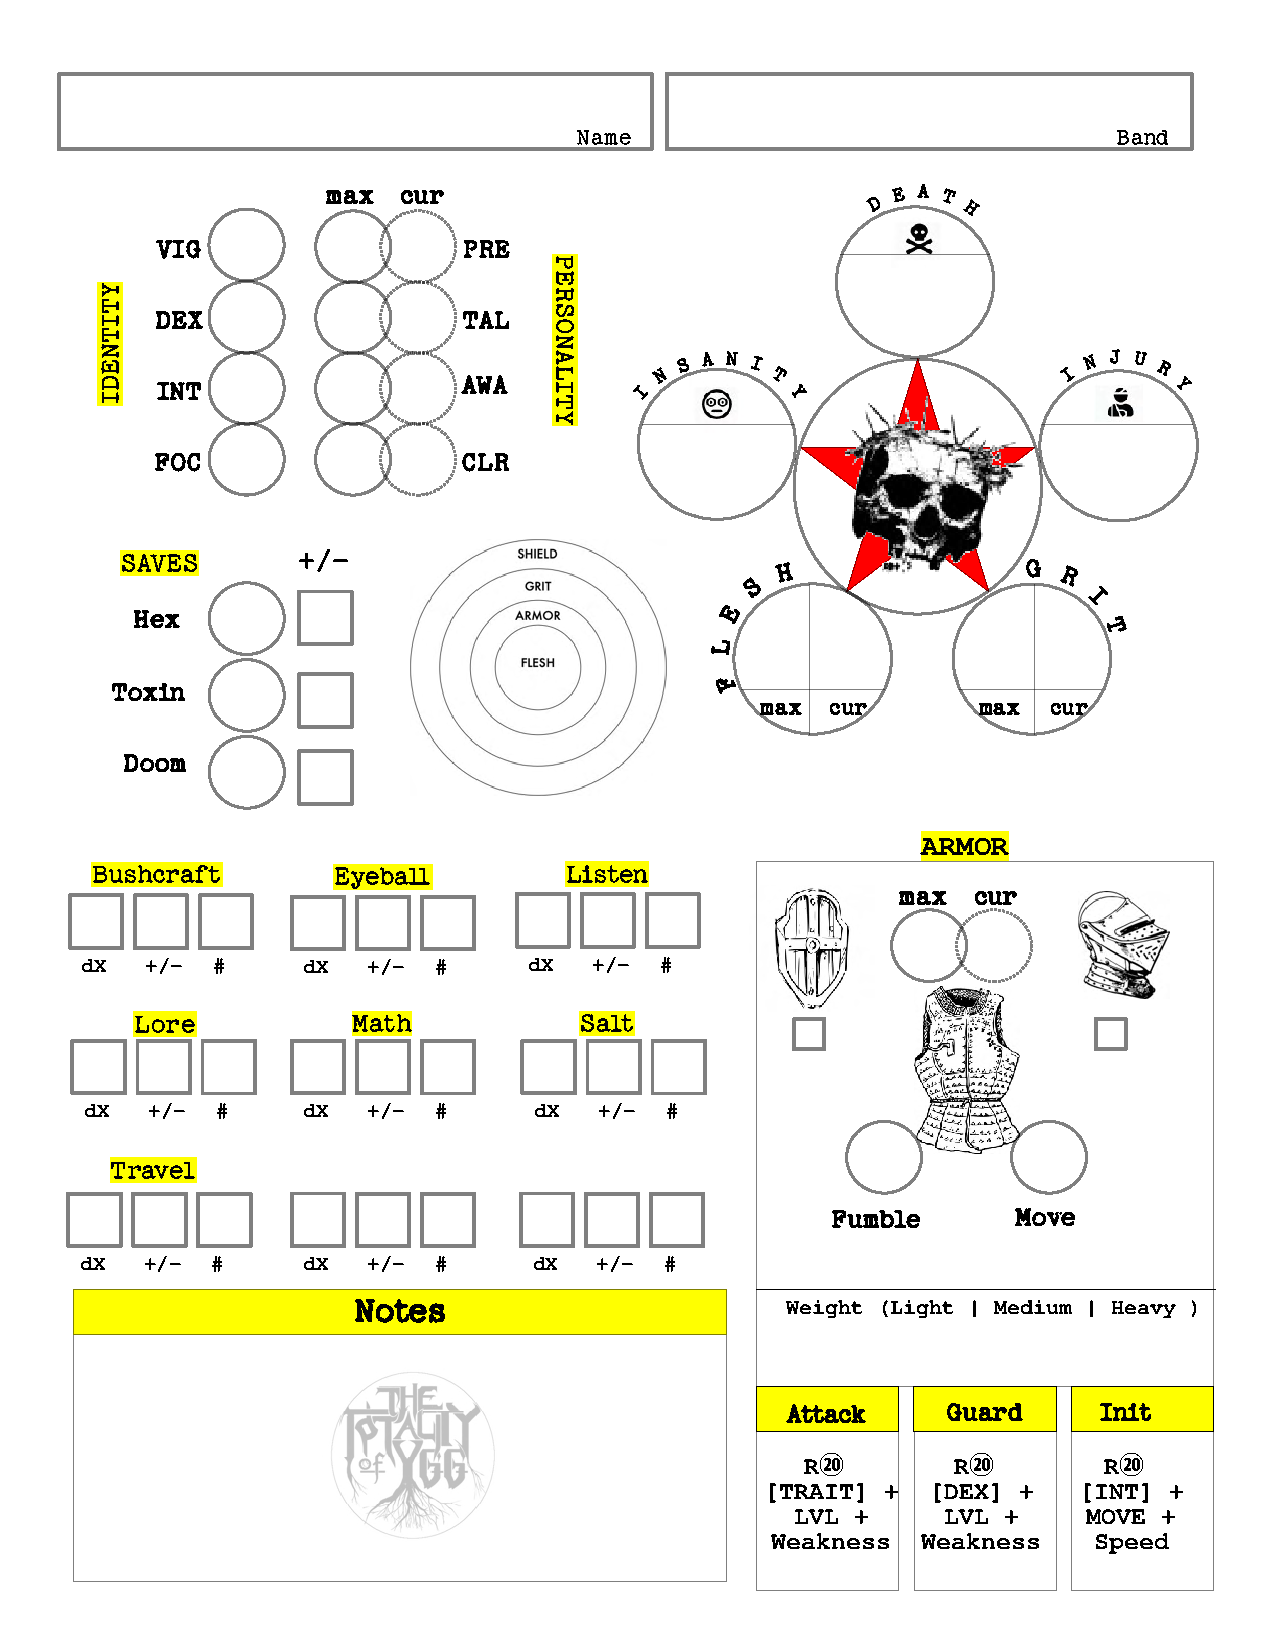
\includepdf[pages=-,pagecommand={},width=\textwidth,link=true,linkname=adventurer-sheet]{pdf/ToY_Character_Sheet.pdf}
  \newpage
  \begin{multicols*}{2}
\mysection{Appendix N}{appendix-n}


\mysubsection{Inspiration}{inspiration}


The Totality of Ygg is an independent work by me (Stefan Antonowicz), and there's no affiliation with any of the links below.  That said, this work wouldn't have been possible without the embarrassment of riches provided by these folks.

\myhighlight{Blogs and Games}{blogs-and-games}

\mybullet {
  \item \href{https://www.lotfp.com/store/}{James Raggi's Lamentations of the Flame Princess}
  \item \href{https://goodman-games.com/dungeon-crawl-classics-rpg/}{Joseph Goodman's "Dungeon Crawl Classics"}
  \item \href{https://the-black-hack.jehaisleprintemps.net/}{David Black's "The Black Hack"}
  \item \href{https://www.soulmuppet.co.uk/products}{Z. Cox's "Best Left Buried"}
  \item \href{https://www.wizardthieffighter.com/}{Luka Rejec's "Ultraviolet Grasslands"}
  \item \href{http://falsemachine.blogspot.com/}{Patrick Stuart's “False Machine”}
  \item \href{http://questingblog.com/}{Ben Milton's "Questing Beast"}
  \item \href{https://theangrygm.com/}{Scott Rehm's "The Angry GM"}
  \item \href{https://www.lastgaspgrimoire.com}{Logan Knight's "Last Gasp Grimoire"}
  \item \href{http://gloomtrain.blogspot.com/}{Mateo Diaz Torres' “Gloomtrain”}
  \item \href{https://coinsandscrolls.blogspot.com/}{Skerple's "Coins and Scrolls"}
  \item \href{http://monstermanualsewnfrompants.blogspot.com/}{Scrap Princess's "Monster Manual Sewn from Pants"}
  \item \href{https://udan-adan.blogspot.com/2016/09/osr-aesthetics-of-ruin.html}{Against the Wicked City}.  The whole blog is great, but I've linked to "Aesthetics of Ruin", which is a must read!
  \item \href{https://golbinpunch.blogspot.com}{Arnold Kemp's "Goblin Punch"}
  \item \href{http://talesofthegrotesqueanddungeonesque.blogspot.com}{Jack Shear's "Tale of the Grotesque \& Dungeonesque"}
  \item \href{https://ageofruins.wordpress.com}{John Carr's "Age of Ruins"}
  \item \href{https://cavegirlgames.blogspot.com/}{Emmy Allen's "Cavegirl's Game Stuff"}
  \item \href{https://thealexandrian.ne}{Justin Alexander's "The Alexandrian"}
  \item \href{https://necroticgnome.com/blogs/news}{Gavin Norman's "Necrotic Gnome"}
  \item \href{https://dungeonofsigns.blogspot.com/}{Gus L's "Dungeon of Signs"}
  \item \href{https://blog.swordfish.press/}{Jacob Hearst's "Swordfish Islands"}
  \item \href{https://permacrandam.blogspot.com/}{"Permanent Cranial Damage"}
  \item \href{https://www.bastionland.com/}{Chris McDowall's "Bastionland"}
  \item All you crazy motherfuckers on /r/osr and Google+ (I'll mourn you til I join you)
}

\myhighlight{Movies and TV}{movies-and-tv}
\mybullet {
  \item Terry Gilliam's "The Brother's Grimm"
  \item Gillermo del Toro's "Crimson Peak"
  \item Showtime's "Penny Dreadful (Season 1)"
  \item Hannah Barbara's "Thundarr the Barbarian"
  \item Gorgonaut's rotoscope shorts (and now \href{https://www.gorgonaut.net/}{The Spine of Night!})
  \item 80s sword and sorcery movies; the Conan trifecta (Barbarian, Destroyer, and Red Sonja); Fire and Ice; Hawk the Slayer; The Beastmaster; Krull; Willow; Dragonslayer; Deathstalker; the Barbarians; Ator: The Fighting Eagle; Hundra; Heavy Metal; etc. etc. 
}

\myhighlight{Authors and Comics}{authors}

China Mieville; Lord Dunsany; Robert E Howard; Clark Ashton Smith; H.P. Lovecraft; Fritz Leiber; E.R. Eddison; Terry Pratchett; \href{https://kenzerco.com/knights-of-the-dinner-table/}{Knights of the Dinner Table}; \href{https://en.wikipedia.org/wiki/Savage_Sword_of_Conan}{SSoC}


\myhighlight{Video Games}{video-games}

Darkest Dungeon; the Dark Souls series; Legends of Grimrock; Urtok: The Desolation; Battle Brothers


\myhighlight{Music}{music}

Extra special thanks to the \href{https://www.youtube.com/channel/UCknVpWR6m2Ijzkqo-aPXs_g}{Stoned Meadows of Doom} and \href{https://soma.fm}{SomaFM}

Sleep; The Sword; Electric Wizard; Kyuss; Kayleth; Master Boot Record; Cracked Machine; Queensr{\UmlautY}che; Weedeater; Sabbath and Maiden; High on Fire; Judas Priest; Planet Cruiser; Thumlock; Eternal Champion; Visigoth; Crypt Sermon; Smoulder

\end{multicols*}

  \newpage
  Creative Commons Attribution-NonCommercial-ShareAlike 4.0 International Public License

\scriptsize {
By exercising the Licensed Rights (defined below), You accept and agree to be bound by the terms and conditions of this Creative Commons Attribution-NonCommercial-ShareAlike 4.0 International Public License ("Public License"). To the extent this Public License may be interpreted as a contract, You are granted the Licensed Rights in consideration of Your acceptance of these terms and conditions, and the Licensor grants You such rights in consideration of benefits the Licensor receives from making the Licensed Material available under these terms and conditions.

Section 1 – Definitions.

    Adapted Material means material subject to Copyright and Similar Rights that is derived from or based upon the Licensed Material and in which the Licensed Material is translated, altered, arranged, transformed, or otherwise modified in a manner requiring permission under the Copyright and Similar Rights held by the Licensor. For purposes of this Public License, where the Licensed Material is a musical work, performance, or sound recording, Adapted Material is always produced where the Licensed Material is synched in timed relation with a moving image.
    Adapter's License means the license You apply to Your Copyright and Similar Rights in Your contributions to Adapted Material in accordance with the terms and conditions of this Public License.
    BY-NC-SA Compatible License means a license listed at creativecommons.org/compatiblelicenses, approved by Creative Commons as essentially the equivalent of this Public License.
    Copyright and Similar Rights means copyright and/or similar rights closely related to copyright including, without limitation, performance, broadcast, sound recording, and Sui Generis Database Rights, without regard to how the rights are labeled or categorized. For purposes of this Public License, the rights specified in Section 2(b)(1)-(2) are not Copyright and Similar Rights.
    Effective Technological Measures means those measures that, in the absence of proper authority, may not be circumvented under laws fulfilling obligations under Article 11 of the WIPO Copyright Treaty adopted on December 20, 1996, and/or similar international agreements.
    Exceptions and Limitations means fair use, fair dealing, and/or any other exception or limitation to Copyright and Similar Rights that applies to Your use of the Licensed Material.
    License Elements means the license attributes listed in the name of a Creative Commons Public License. The License Elements of this Public License are Attribution, NonCommercial, and ShareAlike.
    Licensed Material means the artistic or literary work, database, or other material to which the Licensor applied this Public License.
    Licensed Rights means the rights granted to You subject to the terms and conditions of this Public License, which are limited to all Copyright and Similar Rights that apply to Your use of the Licensed Material and that the Licensor has authority to license.
    Licensor means the individual(s) or entity(ies) granting rights under this Public License.
    NonCommercial means not primarily intended for or directed towards commercial advantage or monetary compensation. For purposes of this Public License, the exchange of the Licensed Material for other material subject to Copyright and Similar Rights by digital file-sharing or similar means is NonCommercial provided there is no payment of monetary compensation in connection with the exchange.
    Share means to provide material to the public by any means or process that requires permission under the Licensed Rights, such as reproduction, public display, public performance, distribution, dissemination, communication, or importation, and to make material available to the public including in ways that members of the public may access the material from a place and at a time individually chosen by them.
    Sui Generis Database Rights means rights other than copyright resulting from Directive 96/9/EC of the European Parliament and of the Council of 11 March 1996 on the legal protection of databases, as amended and/or succeeded, as well as other essentially equivalent rights anywhere in the world.
    You means the individual or entity exercising the Licensed Rights under this Public License. Your has a corresponding meaning.

Section 2 – Scope.

    License grant.
        Subject to the terms and conditions of this Public License, the Licensor hereby grants You a worldwide, royalty-free, non-sublicensable, non-exclusive, irrevocable license to exercise the Licensed Rights in the Licensed Material to:
            reproduce and Share the Licensed Material, in whole or in part, for NonCommercial purposes only; and
            produce, reproduce, and Share Adapted Material for NonCommercial purposes only.
        Exceptions and Limitations. For the avoidance of doubt, where Exceptions and Limitations apply to Your use, this Public License does not apply, and You do not need to comply with its terms and conditions.
        Term. The term of this Public License is specified in Section 6(a).
        Media and formats; technical modifications allowed. The Licensor authorizes You to exercise the Licensed Rights in all media and formats whether now known or hereafter created, and to make technical modifications necessary to do so. The Licensor waives and/or agrees not to assert any right or authority to forbid You from making technical modifications necessary to exercise the Licensed Rights, including technical modifications necessary to circumvent Effective Technological Measures. For purposes of this Public License, simply making modifications authorized by this Section 2(a)(4) never produces Adapted Material.
        Downstream recipients.
            Offer from the Licensor – Licensed Material. Every recipient of the Licensed Material automatically receives an offer from the Licensor to exercise the Licensed Rights under the terms and conditions of this Public License.
            Additional offer from the Licensor – Adapted Material. Every recipient of Adapted Material from You automatically receives an offer from the Licensor to exercise the Licensed Rights in the Adapted Material under the conditions of the Adapter’s License You apply.
            No downstream restrictions. You may not offer or impose any additional or different terms or conditions on, or apply any Effective Technological Measures to, the Licensed Material if doing so restricts exercise of the Licensed Rights by any recipient of the Licensed Material.
        No endorsement. Nothing in this Public License constitutes or may be construed as permission to assert or imply that You are, or that Your use of the Licensed Material is, connected with, or sponsored, endorsed, or granted official status by, the Licensor or others designated to receive attribution as provided in Section 3(a)(1)(A)(i).

    Other rights.
        Moral rights, such as the right of integrity, are not licensed under this Public License, nor are publicity, privacy, and/or other similar personality rights; however, to the extent possible, the Licensor waives and/or agrees not to assert any such rights held by the Licensor to the limited extent necessary to allow You to exercise the Licensed Rights, but not otherwise.
        Patent and trademark rights are not licensed under this Public License.
        To the extent possible, the Licensor waives any right to collect royalties from You for the exercise of the Licensed Rights, whether directly or through a collecting society under any voluntary or waivable statutory or compulsory licensing scheme. In all other cases the Licensor expressly reserves any right to collect such royalties, including when the Licensed Material is used other than for NonCommercial purposes.

Section 3 – License Conditions.

Your exercise of the Licensed Rights is expressly made subject to the following conditions.

    Attribution.

        If You Share the Licensed Material (including in modified form), You must:
            retain the following if it is supplied by the Licensor with the Licensed Material:
                identification of the creator(s) of the Licensed Material and any others designated to receive attribution, in any reasonable manner requested by the Licensor (including by pseudonym if designated);
                a copyright notice;
                a notice that refers to this Public License;
                a notice that refers to the disclaimer of warranties;
                a URI or hyperlink to the Licensed Material to the extent reasonably practicable;
            indicate if You modified the Licensed Material and retain an indication of any previous modifications; and
            indicate the Licensed Material is licensed under this Public License, and include the text of, or the URI or hyperlink to, this Public License.
        You may satisfy the conditions in Section 3(a)(1) in any reasonable manner based on the medium, means, and context in which You Share the Licensed Material. For example, it may be reasonable to satisfy the conditions by providing a URI or hyperlink to a resource that includes the required information.
        If requested by the Licensor, You must remove any of the information required by Section 3(a)(1)(A) to the extent reasonably practicable.
    ShareAlike.

    In addition to the conditions in Section 3(a), if You Share Adapted Material You produce, the following conditions also apply.
        The Adapter’s License You apply must be a Creative Commons license with the same License Elements, this version or later, or a BY-NC-SA Compatible License.
        You must include the text of, or the URI or hyperlink to, the Adapter's License You apply. You may satisfy this condition in any reasonable manner based on the medium, means, and context in which You Share Adapted Material.
        You may not offer or impose any additional or different terms or conditions on, or apply any Effective Technological Measures to, Adapted Material that restrict exercise of the rights granted under the Adapter's License You apply.

Section 4 – Sui Generis Database Rights.

Where the Licensed Rights include Sui Generis Database Rights that apply to Your use of the Licensed Material:

    for the avoidance of doubt, Section 2(a)(1) grants You the right to extract, reuse, reproduce, and Share all or a substantial portion of the contents of the database for NonCommercial purposes only;
    if You include all or a substantial portion of the database contents in a database in which You have Sui Generis Database Rights, then the database in which You have Sui Generis Database Rights (but not its individual contents) is Adapted Material, including for purposes of Section 3(b); and
    You must comply with the conditions in Section 3(a) if You Share all or a substantial portion of the contents of the database.

For the avoidance of doubt, this Section 4 supplements and does not replace Your obligations under this Public License where the Licensed Rights include other Copyright and Similar Rights.

Section 5 – Disclaimer of Warranties and Limitation of Liability.

    Unless otherwise separately undertaken by the Licensor, to the extent possible, the Licensor offers the Licensed Material as-is and as-available, and makes no representations or warranties of any kind concerning the Licensed Material, whether express, implied, statutory, or other. This includes, without limitation, warranties of title, merchantability, fitness for a particular purpose, non-infringement, absence of latent or other defects, accuracy, or the presence or absence of errors, whether or not known or discoverable. Where disclaimers of warranties are not allowed in full or in part, this disclaimer may not apply to You.
    To the extent possible, in no event will the Licensor be liable to You on any legal theory (including, without limitation, negligence) or otherwise for any direct, special, indirect, incidental, consequential, punitive, exemplary, or other losses, costs, expenses, or damages arising out of this Public License or use of the Licensed Material, even if the Licensor has been advised of the possibility of such losses, costs, expenses, or damages. Where a limitation of liability is not allowed in full or in part, this limitation may not apply to You.

    The disclaimer of warranties and limitation of liability provided above shall be interpreted in a manner that, to the extent possible, most closely approximates an absolute disclaimer and waiver of all liability.

Section 6 – Term and Termination.

    This Public License applies for the term of the Copyright and Similar Rights licensed here. However, if You fail to comply with this Public License, then Your rights under this Public License terminate automatically.

    Where Your right to use the Licensed Material has terminated under Section 6(a), it reinstates:
        automatically as of the date the violation is cured, provided it is cured within 30 days of Your discovery of the violation; or
        upon express reinstatement by the Licensor.
    For the avoidance of doubt, this Section 6(b) does not affect any right the Licensor may have to seek remedies for Your violations of this Public License.
    For the avoidance of doubt, the Licensor may also offer the Licensed Material under separate terms or conditions or stop distributing the Licensed Material at any time; however, doing so will not terminate this Public License.
    Sections 1, 5, 6, 7, and 8 survive termination of this Public License.

Section 7 – Other Terms and Conditions.

    The Licensor shall not be bound by any additional or different terms or conditions communicated by You unless expressly agreed.
    Any arrangements, understandings, or agreements regarding the Licensed Material not stated herein are separate from and independent of the terms and conditions of this Public License.

Section 8 – Interpretation.

    For the avoidance of doubt, this Public License does not, and shall not be interpreted to, reduce, limit, restrict, or impose conditions on any use of the Licensed Material that could lawfully be made without permission under this Public License.
    To the extent possible, if any provision of this Public License is deemed unenforceable, it shall be automatically reformed to the minimum extent necessary to make it enforceable. If the provision cannot be reformed, it shall be severed from this Public License without affecting the enforceability of the remaining terms and conditions.
    No term or condition of this Public License will be waived and no failure to comply consented to unless expressly agreed to by the Licensor.
    Nothing in this Public License constitutes or may be interpreted as a limitation upon, or waiver of, any privileges and immunities that apply to the Licensor or You, including from the legal processes of any jurisdiction or authority.

Creative Commons is not a party to its public licenses. Notwithstanding, Creative Commons may elect to apply one of its public licenses to material it publishes and in those instances will be considered the “Licensor.” The text of the Creative Commons public licenses is dedicated to the public domain under the CC0 Public Domain Dedication. Except for the limited purpose of indicating that material is shared under a Creative Commons public license or as otherwise permitted by the Creative Commons policies published at creativecommons.org/policies, Creative Commons does not authorize the use of the trademark “Creative Commons” or any other trademark or logo of Creative Commons without its prior written consent including, without limitation, in connection with any unauthorized modifications to any of its public licenses or any other arrangements, understandings, or agreements concerning use of licensed material. For the avoidance of doubt, this paragraph does not form part of the public licenses.

Creative Commons may be contacted at creativecommons.org.

}


} %end
